\section{Introduction}
Let $(X,g)$ be a space-time and $p\in X$.  One structure that can be associated to a space-time is the space $\mathcal{N}$ of all light rays on the manifold.    To a point $p$ in the manifold one associates the sphere in $\mathcal{N}$ of light rays passing through $p$, which we call its \emph{sky} and denote by $\mathcal{O}_p$.  The space of all skies is called the \emph{sky space} of $X$ and is denoted $SKY(X)$.  The two types of refocusing are related to  properties of the mapping $p\rightarrow \mathcal{O}_p$.  If a space-time is not strongly refocusing then the map is injective.  Furthermore if a strongly causal $X$ is not refocusing Low \cite{LowNull} showed that the map is a diffeomorphism.

The definition of refocusing was first formulated by Low when he was studying the space of light rays of a space-time.  In fact, he proposed three different definitions of refocusing in \cite{LowCS}, \cite{LowSS} and \cite{LowNull}.  The proof of the statement that these definitions are equivalent can be found in the work of Kinlaw \cite{Kinlaw}.  This established the definition of refocusing that we will use in this paper.

After establishing the definitions it is natural to consider whether examples exist of space-times that are strongly refocusing but not refocusing.  In this paper we prove the following result:

\begin{prop} \label{mainProp}
A $1+1$-dimensional oriented, time oriented, refocusing space-time is also strongly refocusing.
\end{prop}

Other related questions were previously explored by Kinlaw \cite{Kinlaw}.  He constructed the first example of a globally hyperbolic space-time which is refocusing but not strongly refocusing at every point in a Cauchy surface.  Using the Poincare conjecture proved by Perlman, he was also able to prove that any globally hyperbolic refocusing space-time of dimension $\leq 4$ admits a strongly refocusing metric.

These results provide the basis for our investigation, as they also aim to answer if and when there are examples of space-times that are refocusing but are not strongly refocusing.

\section{Definitions} 
In this section we will provide the definitions that we use throughout the paper.  We begin with the definitions of strong refocusing and refocusing.
\begin{defin} \label{srefoc}
A space-time $(X, g)$ is \emph{strongly refocusing} at $p\in X$ if there exists $q\neq p \in X$ such that all the light rays passing through $q$ also pass through $p$.  We say $X$ is \emph{strongly refocusing} if there exists $p\in X$ such that $X$ is strongly refocusing at $p$.
\end{defin}

\begin{rem}
In Low's work refocusing was considered only for strongly causal space-times.  In this work we do not use this assumption.
\end{rem}

In order to define refocusing we weaken the conditions of strong refocusing.  Low initially proposed three definitions for refocusing, and for strongly causal space-times they were proven to be equivalent by Kinlaw \cite{Kinlaw}.  We will use the following definition:
\begin{defin} \label{refoc}
A space-time $(X, g)$ is \emph{refocusing} at $p\in X$ if there exists an open neighborhood $V$ of $p$ such that for all open $U\subset V$ with $x\in U$ there exists $y\notin V$ such that all null geodesics passing through $y$ also pass through $U$.
\end{defin}

From these definitions it is clear that any strongly refocusing space-time is  refocusing.


\subsection{Right and Left Null Geodesics}
For a $1+1-$dimensional oriented, time-oriented space-time $X$, each null geodesic in $X$ can be classified into one of two types.  Let $\gamma$ be a null geodesic, and let $Y$ be any timelike future pointing vector field.  The pair $\gamma '(t)$ and $Y(\gamma(t))$ are linearly independent, and thus form a basis for $T_{\gamma(t)}X$ for any $p\in X$. 

\begin{defin}
Let $\gamma$ be a null geodesic of $X$.  We say that $\gamma$ is \emph{left-facing} if the pair $\gamma '(t)$ and $Y(\gamma(t))$ give a negative orientation for all $t$ and \emph{right-facing} if they form a positive orientation for all $t$. 
\end{defin}

\begin{rem}
\begin{enumerate}
\item Every null geodesic is either left facing or right facing.
\item Each point $p\in X$ has exactly two null geodesics passing through it, one of which is left facing and one of which is right facing.  We denote by $\rho_x$ the right facing null geodesic starting at $x$ and by $\lambda_x$ the left facing null geodesic starting at $x$.
\item It is impossible for two right-facing or two left-facing geodesics to intersect.
\end{enumerate}
\end{rem}



\section{Proof of \ref{mainProp}}
In this section we will prove Proposition \ref{mainProp}.  Throughout the section let $(X, g)$ be an oriented, time-oriented $1+1$ dimensional space-time.  Recall that for any $p,q\in X$, $I^\pm(p)$ denotes the chronological future/past of $p$ and $I(p,q) = I^+(p) \cap I^-(q)$.

Suppose that we have refocusing at $x\in X$.  Again, let $Y$ be a future facing timelike vector field on $X$.  Since $X$ is refocusing at $x$ we have a neighborhood $W$ of $x$ such that for any open $U\subset W$ with $x\in U$ there exists $y\notin W$ where all the null geodesics passing through $y$ also pass through $U$.  

We begin by constructing a neighborhood of $x$ where we will force strong refocusing to occur.  Choose $z_1, z_2\in W$ such that $I(z_1, z_2) \subset W$ is a globally hyperbolic, normal neighborhood of $x$.  Choose $y \notin W$ such that $\lambda_y$ and $\rho_y$ both pass through $I(z_1, z_2)$.  Let $p\in \mbox{Im}(\lambda_y) \cap I(z_1, z_2)$ and $q\in \mbox{Im}(\rho_y) \cap I(z_1, z_2)$, as in figure \ref{figure2.fig}.

\begin{figure}[hbtp]
	\centering
	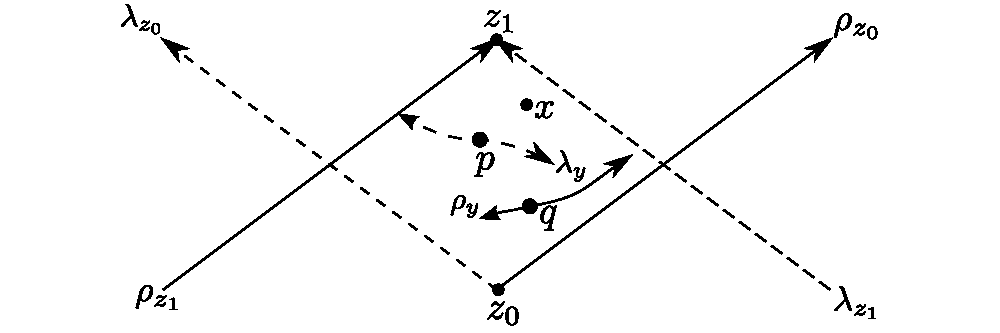
\includegraphics[width=12cm]{refocussingNbhd}
	\caption{A diagram of $I(z_0, z_1)$}
	\label{figure2.fig}
\end{figure}

Since this is a normal neighborhood, the geodesics must be well behaved and thus $\lambda_y$ must intersect $\rho_y$ in $I(z_1, z_2)$.  Thus $X$ is strong refocussing at $y$.

\begin{rem}
All known examples of refocusing higher dimensional space-times are also strongly refocusing.  Whether this is always the case remains an open question.
\end{rem}

